\section*{Experiments\label{exp}}
\subsection{Experimental Setup}
\subsubsection{Datasets}
We evaluated SharpView extensively on two types of datasets: complicated single 3D objects downloaded online\footnote{\url{https://www.cgtrader.com}} (3 single 3D objects with number of vertices varying from 0.9M to 3.6M) and large 3D indoor scenes (sizes varying from $30m^2$ to $100m^2$) from the habitat Replica dataset~\cite{replica19arxiv}.
% Since the former two datasets are bare 3D scenes without standard sequences of views provided, we generate random sequences of views for them.
% We generate 2500 views for each scene in the former two dataset and we use the default sequence of views provided in ICL-NUIM where simulated noise was added to simulate $\bm{v}$.
% The single 3D objects are complicated models of a drone, a motorcycle and a robot with number of vertices varying from 0.9M to 3.6M and we generate 2500 random views of each object by positioning the camera on a sphere with fixed radius surrounding the 3D object and the camera pointing towards the center of the 3D object.
% The Replica datasets is a large scale indoor scene dataset commonly used in 3D reconstruction tasks that feature complex indoor scenes with sizes varying from $30m^2$ to $100m^2$.
We randomly generate 2500 navigable views for both datasets except that in the 3D object dataset, the camera is positioned on a sphere with fixed radius surrounding the 3D object and the camera pointing towards the center of the 3D object and in Replica dataset, the camera randomly roams in the indoor scene.
% All used datasets are provided with ground-truth 3D mesh models for evaluation.
Our chosen datasets cover the common use cases of 3D reconstruction and suffice to reveal the ability of our proposed method SharpView to generalize its performance in various situations.

We use the these sequences of views to simulate $v$ for each scene, 
and at the beginning, we initialize $\bm{v_n}$ with a view randomly selected from $\bm{v}$ and the underlying 3D reconstruction method trains its latent codes with $\bm{v_n}$.
The size of candidate views for NBV selection in our evaluation is 100 and the candidate views are randomly sampled from unvisited views (satisfy $v\in\bm{v}\land v\notin \bm{v_n}$).
% To generate candidate views from $\bm{v}$., we randomly select 100 unvisited views (satisfy $v\in\bm{v}\land v\notin \bm{v_n}$) and NBV process estimates the information gain of each view without the knowledge of the actual RGBD image and decides to visit the view of highest information gain.
% At the beginning, $\bm{v_n}$ is initialized with a random view from $\bm{v}$ and we cease the iteration of NBV selection when the size of $\bm{v_n}$ reaches 300.


\subsubsection{Metrics}
We mainly follow the metrics used in BNV Fusion~\cite{li_bnv-fusion_2022} for end-to-end evaluation.
Specifically, Accuracy (referred to as Accu.) measures the fraction (one hundred percentage) of points from the reconstructed mesh that are within a preset distance (2cm in our evaluation) from the ground-truth mesh.
Completeness (referred to as Comp.) calculates the fraction of points from the groundtruth mesh that are within a preset distance (2cm) from the point in the reconstructed mesh.
F1 score (referred to as F1) is the harmonic mean of accuracy and completeness, which is the major metric we use to quantify the overall reconstruction quality as it balances between completeness and accuracy.
% Other metrics we used is Peak Signal-to-Noise Ratio (PSNR) that follows the equation of $PSNR=10\cdot\log_{10}(\frac{MAX^2}{MSE})$, which is commonly used~\cite{avidan_activenerf_2022,jin_neu-nbv_2023} to measure the similarity between the groundtruth image and the image rendered from implicit model.
% $MAX$ is the maximal possible value on the image and $MSE$ is the mean square error between the estimated image and groundtruth image.
% We use PSNR to estimate how much the current reconstructed model is similar to the groundtruth from a certain view, and lower PSNR represents more differences, but not always more space for improvement of the reconstructed model which we will discuss later.

\subsubsection{Workload}
We choose a state-of-the-art grided implicit 3D reconstruction method, BNV Fusion~\cite{li_bnv-fusion_2022} as our major workload.
Since BNV Fusion mainly targets at recovering the accurate shape of the scene and does not make use of the RGB part of the image, we are considering depth measurements only in our evaluation but we believe the results can generalize to wider scope of measurements and tasks.
The aforementioned $MAX$ is the maximal depth value we measure from the camera, which is set to be 3 meters following the default setting of~\cite{li_bnv-fusion_2022}.
The voxel size (proportional to the size of the local geometry for a local latent code) for the single 3D objects is 1cm to extract finer details and the voxel size for the Replica dataset is 2cm to save GPU memory and map a large scene.
We also use the default hyper-parameters in its demo setting and use their released checkpoint for the encoder and the decoder.
It is notable that the latent codes $\theta$ are only trained for 10 iterations on an NBV $v_{n+1}$ being input to $\bm{v_n}$ in BNV Fusion.
% The only modification we made on BNV Fusion is to explicitly group their local latent codes as a matrix to simplify our implementation of SharpView.

\subsubsection{Testbed}
The testbed we use is a commodity laptop equipped with an Nvidia 2070 8GB laptop GPU, an Amd Ryzen 3600 CPU and 16GB RAM.

\subsubsection{Baselines}
We compare SharpView with two naive baselines (Random and Max Distance) and an re-implementation (Predict) of prior methods~\cite{shen_stochastic_2021,jin_neu-nbv_2023,ran_neurar_2023,avidan_activenerf_2022} that predicts the uncertainty of model outputs for NBV selection.
Specifically, Random (referred to as Rand.) randomly selects a view from the candidate views as NBV.
Max Distance (referred to as MaxDist.) selects a view from the candidate views as NBV whose shortest distance to anyone in $\bm{v_n}$ is the longest.
In Predict (referred to as Pred.), we added an extra model head to the decoder of BNV Fusion which predicts the uncertainty $\sigma$ of the model output (depth measurement $d$).
We set the loss function used during training of Pred. following the patterns of loss functions commonly used in these methods~\cite{shen_stochastic_2021,jin_neu-nbv_2023,ran_neurar_2023,avidan_activenerf_2022}: 
\begin{equation*}
    L = \frac{1}{R} \sum_{r=0}^R  (\log \sigma_r + \frac{(d_r-\bar{d}_r)^2}{\sigma_r^2})
\end{equation*}
where $R$ is the number of pixels in an input image and $\bar{d}$ is the groundtruth depth measurement.
We use the same information gain estimation pipeline for Pred. as SharpView, except that we render images $I''$ for Pred. through inference for the model output.

All scripts to generate the datasets and calculate the metrics are included in our released repository.

\subsection{End-to-End Results}
\begin{table*}[htb]
    \centering
    \caption{End-to-end results on circulated sampling on 3D models. Numbers in the first row represents the size of current $\bm{v_n}$. Time of the last colum is the time duration from $n=0$ to $n=90$.\label{model}}
    \begin{tabular}{|c|c|c|c|c|c|c|c|c|c|c|c|c|c|c|c|c|c|}
        \hline
        \multirow{2}{*}{Methods} & \multirow{2}{*}{Scene} & \multicolumn{3}{c|}{n=30}& \multicolumn{3}{c|}{n=60}& \multicolumn{3}{c|}{n=90} & Time$\downarrow$\\ \cline{3-11} 
        &  & Accu.$\uparrow$ & Comp. $\uparrow$& F1 $\uparrow$ & Accu.$\uparrow$ & Comp. $\uparrow$& F1 $\uparrow$& Accu. $\uparrow$& Comp. $\uparrow$& F1 $\uparrow$& (m) \\ \hline
        \multirow{3}{*}{SharpView} & drone & 54.585& 39.454& 47.020
            & 53.806& 43.085& 48.446
                & 54.113& 45.088& 49.601 & 6\\    \cline{2-12}
            & motorcycle & 73.246& 55.778& 64.512
            & 71.947& 58.631& 65.289
                & 71.179& 59.932& 65.555& 5\\                 \cline{2-12}
            & robot & 54.026& 34.901& 44.464
            & 53.744& 37.977& 45.861
                & 53.419& 39.584& 46.502& 5\\                      \hline
        \multirow{3}{*}{Rand.} & drone &53.975& 37.471& 45.723
            & 53.761& 42.163& 47.962
                & 53.578& 44.295& 48.937 & 6\\    \cline{2-12}
            & motorcycle & 73.261& 56.022& 64.641
            & 71.999& 58.471& 65.235
                & 70.337& 59.763& 65.050 & 4\\                 \cline{2-12}
            & robot & 55.015& 35.970& 45.492
            & 53.989& 38.786& 46.387
                & 53.911& 39.856& 46.884 & 5\\                      \hline
        \multirow{3}{*}{MaxDist.} & drone & 53.949& 41.016& 47.483
            & 53.648& 44.611& 49.130
                & 53.794& 46.477& 50.135 & 6\\    \cline{2-12}
            & motorcycle & 73.072& 56.002& 64.537
            & 71.069& 58.791& 64.929
                &70.167& 60.103& 65.135 & 5\\                 \cline{2-12}
            & robot &54.466& 36.070& 45.268
            & 53.839& 39.006& 46.422
                &53.670& 40.161& 46.916 & 5\\                      \hline
        \multirow{3}{*}{Pred.} & drone &53.677& 38.836& 46.257
            & 53.426& 42.904& 48.164
                & 53.022& 44.620& 48.821 & 33\\    \cline{2-12}
            & motorcycle & 72.430& 55.086& 63.758
            & 70.097& 57.478& 63.788
                & 69.142& 58.558& 63.850 & 14\\                 \cline{2-12}
            & robot & 54.526& 36.425& 45.475
            & 54.084& 38.477& 46.281
                &53.151& 39.261& 46.206 & 27\\                      \hline
    \end{tabular}
\end{table*}
\subsubsection{Next Best View for Single 3D Objects}
However the design and implementation, we regret to report that we did not get the results we wanted, but we want to report the interesting findings we got during experiments and we are eager to communicate with reviewers.
Table~\ref{model} shows the comparison on single 3D objects and the differences among all settings are marginal.
% Under the same size of $\bm{v_n}$ (denoted as $n$), both SharpView and Pred. outperform the naive baselines with TODO\% $\sim$ TODO \% advantage in F1 with the guidance of synaptic dynamics or model output uncertainty, but 
% SharpView highlights TODO\% $\sim$ TODO\% higher F1 than all the baselines, revealing that the selection of NBV in SharpView has higher contribution to the model improvement.
% To reach the same F1 as SharpView in the TODO scenes when $n=TODO$ , Pred. even required doubled size of $\bm{v_n}$.
% SharpView also highlights almost the same time consumption to estimate and collect $n=90$ views as the naive baselines, while Pred. increase the time consumption by TODO X.
It is notably observed that as the increase of Comp., Accu. is decreasing as $n$ increases.
Such observation also holds for the baselines as shown in Table~\ref{model}, which is an evidence for the capacity limit of local latent codes as discussed below.

To understand the decrease of Accu. as $n$ increases, let us contrast it with the increase of Comp. as $n$ increases.
In the setting of evaluation on single 3D objects, the dimensions of freedom of the camera is reduced to 2 dimensions by fixing the camera's pointing direction and fixing its positioning to a sphere.
As a result, most part of the whole surfaces of a 3D object can be quickly covered (over 50\% Comp. in the motorcycle case) with a comparatively small $n=30$.
As more views are being input, more new local geometries not included in the previous training dataset are also input, and the local latent codes are trained to attend to them, accounting for the increase of Comp.
But when the complexity of local geometries exceed the capacity of local latent codes, the local latent codes would have to compromise among the local geometries to reach global optimal of the loss function by not accurately mapping all the local geometries, but rather their medians, which accounts for the decrease of Accu.

% In such circumstances, the uncertainty of model output related to these local latent codes tends to increase (larger $\sigma$) because the model output slightly disagrees with the groundtruth image, but more input views to train these local latent codes can barely improve Accu. (decrease $\sigma$) since these local latent codes has approached their global optimal.
% Thus NBV selection based on model output uncertainty tends to be stuck at these local latent codes with no improvement of the reconstructed model, while SharpView is able to discover and avoid such local latent codes by calculating a higher certainty $c_j^{n}$ through the synaptic dynamics dynamics during training of the local latent codes, which explains TODO\% $\sim$ TODO\% higher F1 advantages of SharpView over Pred.

\subsubsection{Next Best View for Large Scale Indoor Scenes}
Here we present the comparison results of SharpView and the baselines over large scale indoor scenes from Replica dataset.
The differences among all settings are marginal. But the same phenomenon of capacity limit of local latent codes remains, where Accu. decreases as Comp. increases.

\begin{table*}[htb]
    \centering
    \label{habitat}
    \caption{End-to-end results on free sampling on habitat indoor scenes.}
    \begin{tabular}{|c|c|c|c|c|c|c|c|c|c|c|c|c|c|c|c|c|c|}
        \hline
        \multirow{2}{*}{Methods} & \multirow{2}{*}{Scene} & \multicolumn{3}{c|}{n=100}& \multicolumn{3}{c|}{n=200}& \multicolumn{3}{c|}{n=300} & Time $\downarrow$\\ \cline{3-11} 
        &  & Accu.$\uparrow$ & Comp. $\uparrow$& F1 $\uparrow$ & Accu.$\uparrow$ & Comp. $\uparrow$& F1 $\uparrow$& Accu. $\uparrow$& Comp. $\uparrow$& F1 $\uparrow$& (m) \\ \hline
        \multirow{3}{*}{SharpView} & frl\_apartment\_1 & 44.498& 39.618& 42.058
            & 44.142& 42.514& 43.328
                & 43.740& 42.636& 43.188 & 65\\    \cline{2-12}
            & hotel\_0 & 54.627& 53.806& 54.217
            & 53.792& 54.839& 54.316
                & 53.520& 54.970& 54.245 & 29\\                 \cline{2-12}
            & room\_1 &74.267 & 75.044  & 74.655
            & 71.317 & 76.139 & 73.728
                & 70.147 & 76.035 & 73.091 & 23\\                      \hline
        \multirow{3}{*}{Rand.}  & frl\_apartment\_1 &45.050& 39.418& 42.234
        & 44.084& 42.332& 43.208
            & 43.565& 42.634& 43.099 & 55\\    \cline{2-12}
            & hotel\_0 & 54.469& 53.947& 54.208
            & 53.615& 55.190& 54.402
                & 53.377& 55.616& 54.497& 29\\                 \cline{2-12}
            & room\_1 &73.011& 74.304& 73.657 
            & 70.025& 75.225& 72.625
                &67.986& 75.113& 71.549 & 23 \\                      \hline
        \multirow{3}{*}{MaxDist.} & frl\_apartment\_1 & 44.920 & 40.532 & 42.726
        & 44.142 & 42.865 & 43.504
            & 43.484 & 42.870 & 43.177 & 57\\    \cline{2-12}
            & hotel\_0 & 54.238& 54.700& 54.469
            & 53.538& 55.732& 54.635
                & 53.181& 55.766& 54.473 & 29\\                 \cline{2-12}
            & room\_1 & 73.274 & 75.941 & 74.607
            &70.401 & 76.082 & 73.242 &
            68.132 & 75.633 & 71.883& 27\\                      \hline
        \multirow{3}{*}{Pred.} & frl\_apartment\_1 & 44.636& 38.860& 41.748
            & 44.106& 42.070& 43.088
                & 43.992& 42.584& 43.288 & 89\\    \cline{2-12}
            & hotel\_0 & 54.132& 54.407& 54.270
            & 53.819& 54.947& 54.383
                & 53.373& 55.375& 54.374 & 57\\                 \cline{2-12}
            & room\_1 & 75.008& 73.620& 74.314
            & 73.627& 74.468& 74.047
                & 72.642& 74.803& 73.722& 69\\                      \hline
    \end{tabular}
\end{table*}
% \subsection{Breakdown}
% % \subsection{Ablation Study}
% \begin{figure}
%     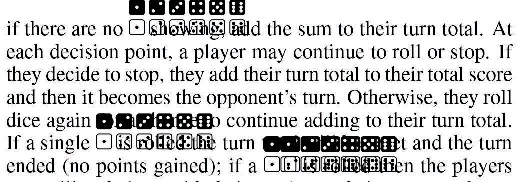
\includegraphics{figure1.pdf}
%     \caption{heading\label{Breakdown}}
% \end{figure}
% To further understand the above results, we breakdown the training time statistics of SharpView and Pred. and analyze the correlation between their estimated information gain with the actual improvement of reconstructed models.
% Specifically, given a view $v_{n+1}$ being input as the NBV for training the latent codes, we record the PSNR estimated for $v_{n+1}$ before optimization and after optimization, which quantifies the information extracted from $v_{n+1}$.
% We also recorded $\Delta$F1 before optimization and after optimization to record the improvement of the reconstructed model.

% We contrast the runtime estimated information gain for $v_{n+1}$ and the recorded PSNR and $\Delta$F1 in Fig.~\ref*{Breakdown} in the single 3D object drone setting.
% We can observe both our information gain estimation based on certainty estimation (see equation~(\ref*{ourgain}) and information gain estimation based the uncertainty estimation of model output in Pred. are linearly correlated with PSNR before optimization.
% It implies that both methods successfully discover where the reconstructed model disagrees with the groundtruth, but in Pred. the information gain estimation is barely correlated with $\Delta$F1 due to the interference of capacity limit of local latent codes as discussed above, while in SharpView the linear correlation remains, confirming the effectiveness of SharpView in modelling the possible model improvement.

\subsection{Limitations and Discussions}
A possible reason for the unfavorable results can be due to our training setting, where the model is trained continuously on a single image instead of on all visited images, which leads to forgetting.
We will better our setting and continue to work.
A limitation of our proposed method is that while we can distinguish local latent codes that can be improved, we select the viewing direction to improve these latent codes with simple heuristics instead of comparing the inference results for each candidate viewing direction as the prior work.
On one hand this design choice saves the computation-intensive inference, on the other hand we have demonstrated above that the uncertainty estimation through inference failed to model the possible improvement of local latent codes.
We leave the development for a more refined searching strategy for viewing direction as future work.
It is also notable that although grided implicit 3D reconstruction is the only task we are targeted in this paper, its idea of decomposition would have a broader impact on machine learning tasks modelling the world such as recognition and segmentation.
It shows an efficient way to implement in machine learning the most natural process of human learning, which decomposes a complex task to simple subtasks and solves each subtasks individually, and would nurture the development of more similar decomposition-based machine learning paradigms, where our proposed method would also benefit.

